% ======================================================================
% talk-pagestack.tex
%
% A stack of A4 pages for representing the SMT-LIB standard visually.
% Self-contained demo -- build with:  latexmk -lualatex talk-pagestack.tex
%
% TO LIFT INTO talk.tex / talk-ijcar.tex:
%   Neither talk currently loads TikZ, so add to the preamble:
%       \usepackage{tikz}
%       \usetikzlibrary{shadows.blur, overlay-beamer-styles, calc, positioning}
%   then copy the \newcommand + \tikzset block below and whichever frame
%   you want. Nothing else here is needed.
% ======================================================================
\documentclass[lualatex, compress, 11pt]{beamer}
\usetheme{metropolis}

\usepackage{tikz}
\usetikzlibrary{shadows.blur, overlay-beamer-styles, calc, positioning}
\usepackage{graphicx}

% ---- A4 proportions: 1 : sqrt(2) -------------------------------------
\newcommand{\pgw}{2.4cm}
\newcommand{\pgh}{3.394cm}   % 2.4 * 1.41421

\tikzset{
  a4page/.style={
    draw=black!35, fill=white, line width=0.4pt,
    minimum width=\pgw, minimum height=\pgh, inner sep=0pt,
    blur shadow={shadow blur steps=10, shadow xshift=1.2pt,
                 shadow yshift=-1.6pt, shadow opacity=40}
  },
  ruled/.style={black!22, line width=0.5pt}
}

% Fake body text on the page node named #1, so a blank rectangle reads
% as "a document". Drop this if you use real pages (Frame 4).
\newcommand{\ruledlines}[1]{%
  \foreach \y in {0.55,0.78,...,2.9} {
    \draw[ruled] ($(#1.north west)+(0.22,-\y)$) -- ($(#1.north east)+(-0.22,-\y)$);
  }
}

\begin{document}

% ======================================================================
% 1. Static fan. Pages pivot about a shared bottom-left corner.
%    \rot controls the spread: 8 degrees per page is a gentle fan,
%    15+ starts to look like a hand of cards.
% ======================================================================
\begin{frame}{Static fan}
\centering
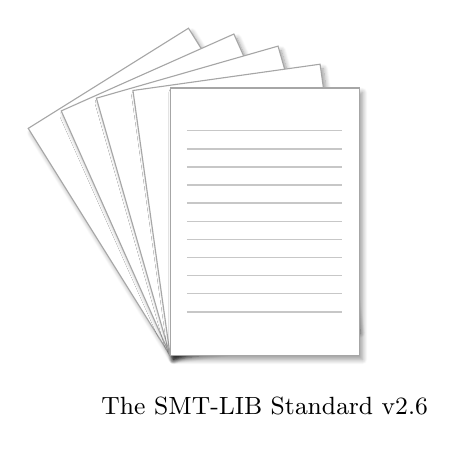
\begin{tikzpicture}
  \foreach \i in {5,4,3,2,1} {
    \pgfmathsetmacro{\rot}{(\i-1)*8}
    \node[a4page, rotate around={\rot:(0,0)}, transform shape,
          anchor=south west, name=p\i] at (0,0) {};
  }
  \ruledlines{p1}
  \node[below=4mm of p1.south] {\small The SMT-LIB Standard v2.6};
\end{tikzpicture}
\end{frame}

% ======================================================================
% 2. Fans out across overlays -- the "animation".
%
%    NOTE the \onslide<1-5>{} line. It is load-bearing: beamer counts a
%    frame's slides by scanning for overlay specs, and inside \foreach it
%    only ever sees the literal "<\i->", which it cannot parse. Without
%    it you get one slide and the fan never opens. Keep the upper number
%    in sync with the number of pages.
% ======================================================================
\begin{frame}{Fans out, one page per click}
\onslide<1-5>{}%
\centering

\begin{tikzpicture}
  \foreach \i in {5,4,3,2,1} {
    \pgfmathsetmacro{\rot}{(\i-1)*8}
    \node[a4page, rotate around={\rot:(0,0)}, transform shape,
          anchor=south west, name=p\i,
          visible on=<\i->] at (0,0) {};
  }
  \ruledlines{p1}
\end{tikzpicture}
\end{frame}

% ======================================================================
% 3. Loose pile -- rotations both ways, jittered offsets. Reads as
%    "a pile of paper on a desk" rather than a deliberate fan.
% ======================================================================
\begin{frame}{Loose pile}
\centering

\begin{tikzpicture}
  \foreach \r/\x/\y in {-9/-0.25/-0.1, 6/0.15/0.05, -3/-0.05/-0.05,
                        2/0.08/0.02, 0/0/0} {
    \node[a4page, rotate=\r, name=q] at (\x,\y) {};
  }
  \ruledlines{q}
\end{tikzpicture}
\end{frame}

% ======================================================================
% 4. REAL pages of the standard. Probably what you actually want:
%    it makes the "this is a 100-page document" point without you
%    having to say it.
%
%    Fetch the PDF into this directory first:
%      wget https://smt-lib.org/papers/smt-lib-reference-v2.7-r2025-07-07.pdf \
%           -O smtlib.pdf
%
%    This frame compiles to nothing until that file exists, so the
%    document always builds.
%
%    PDF page 77 is the model-theoretic semantics (Chapter 5, Logical
%    Semantics of SMT-LIB Formulas) if you want the top sheet to be the
%    part the paper's framing parallels. PDF 55 is a near-blank part
%    divider; avoid it.
% ======================================================================
\IfFileExists{smtlib.pdf}{%
\begin{frame}{The SMT-LIB Standard}
\onslide<1-5>{}%
\centering
\begin{tikzpicture}
  \foreach \i/\pg in {5/40, 4/30, 3/20, 2/10, 1/1} {
    \pgfmathsetmacro{\rot}{(\i-1)*8}
    \node[a4page, rotate around={\rot:(0,0)}, transform shape,
          anchor=south west, name=p\i, visible on=<\i->] at (0,0)
         {\includegraphics[width=\pgw, page=\pg]{smtlib.pdf}};
  }
\end{tikzpicture}
\end{frame}
}{%
\begin{frame}{Real pages of the standard}
  \small Fetch \texttt{smtlib.pdf} into this directory (see the comment in
  \texttt{talk-pagestack.tex}) and this frame renders actual pages of the
  standard instead of this placeholder.
\end{frame}
}

\end{document}
